\chapter{Desenvolvimento do modelo OLAP}
\label{cap:DesenvolvimentoDoModeloOLAP}
%-------------------------------------------------------
% descrever como foi feito o levantamento dos residuos mais interesantes. 
%  Explicar que a lista dos mais presentes foi comparada com uma lista originalmente desenvolvida por um especialista de dominio. 
%  Encontrou se casos que estavam e nao estavam na lista, os que nao apareciam na lista constituem de residuos que se ficam ˜proximos”ao sitio de ligação, mas que na realidade estão fora do sítio.
% descrever como  adicionar novas dimensoes baseadas em novos residuos
%-------------------------------------------------------

Para possibilitar a construção do modelo OLAP, primeiramente foi necessário identificar e definir as questões de negócio que seriam relevantes sob o ponto de vista do especialista de domínio. Em virtude disso, o levantamento destes dados foi feito por meio de entrevistas com os especialistas do LABIO.

A Tabela \ref{tab:questaoNegocio} descreve as questões de negócio que foram identificadas como sendo mais relevantes para execução de análise de experimentos de docagem realizados no LABIO. 

\begin{table}[h]
\caption{Questões de negócio identificadas pelos especialistas com maior relevância para análise de experimentos de docagem}
\label{tab:questaoNegocio}
\centering
\begin{tabular}{@{}ll@{}}
\toprule
\textbf{ } & \multicolumn{1}{c}{\textbf{Questões de maior relevância para a análise de docagem}}		\\ \midrule
\textbf{1.} & Associar um grupo para cada conformação;													\\
\textbf{2.} & Identificar o comportamento das conformações baseado nas métricas de FEB e RMSD;			\\
\textbf{3.} & Identificar conformações/grupos que possuem o maior número de contatos com os ligantes;	\\
\textbf{4.} & Com base no item 3, identificar quais são os resíduos mais importantes;					\\
\textbf{5.} & Com base no item 3, identificar quais grupos possuem melhores valores de FEB e RMSD.		\\ \bottomrule
\end{tabular}
\end{table}

\section{Identificação de métricas}
\label{sec:IdentificacaoDeMetricas}

Durante as entrevistas realizadas, pode-se perceber que informações baseadas nas métricas de FEB e RMSD possuíam grande relevância para responder as questões de negócio. Entretanto foi necessário definir certas propriedades e limitações de valores para adequar os cálculos às necessidades do negócio. Dessa maneira, todas as definições citadas nesta seção foram estabelecidas em conjunto com os especialistas de domínio do LABIO, para que os resultados apresentados pudessem representar a realidade.

O cálculo da FEB é um dos métodos utilizados pelos softwares de docagem que permite avaliar a interação receptor-ligante. Quanto menor for o resultado deste cálculo, mais favorável é a ligação estabelecida. Portanto, o valor estimado da FEB é utilizado como uma das métricas do modelo.

Na maioria dos experimentos, os melhores resultados de FEB são valores negativos. Portanto, qualquer conformação que apresente valores de FEB positivos não foram levados em consideração. Dessa maneira evita-se que os resultados positivos venham a interferir em uma análise futura dos valores agregados de um experimento. 

O cálculo do RMSD é utilizado para obter a distância média entre os átomos. Nos experimentos de docagem, este cálculo é feito para comparar o posicionamento inicial do ligante, geralmente estipulada pelo especialista de domínio, com o posicionamento final após a execução da docagem. Neste caso, o RMSD é considerado como uma métrica para a modelagem.

Tanto a FEB quando o RMSD dão uma visão para o especialista de quão satisfatório foi o processo de docagem para uma determinada iteração. Enquanto a FEB mede a qualidade da docagem no aspecto termodinâmico da questão, o RMSD tem como natureza avaliar geometricamente como estão dispostas as moléculas do resíduo e do ligante.

Além disso, para ser possível responder ao item 3 da Tabela \ref{tab:questaoNegocio}, foi necessário incluir uma métrica para contabilizar o número de contatos entre o ligante e um resíduo da molécula receptora. 

Um contato pode ser identificado pelo cálculo da medida em {\AA}ngstr\"om ({\AA}) entre os átomos do resíduo do receptor e do ligante. Ou seja, para cada resíduo do receptor \emph{R} é calculada a distância Euclidiana entre todos seus átomos e os átomos de um ligante \emph{L}. Sendo $R=(r_{x},r_{y},r_{z})$ representando as coordenadas dos átomos dos resíduos do receptor, e $L=(l_{x},l_{y},l_{z})$ representando as coordenadas dos átomos do ligante, o cálculo da distância se dá pela equação \ref{eqt:distEuclid}.

\begin{equation}
\label{eqt:distEuclid}
	d(R,L)=\sqrt{(r_{x}-l_{x})^{2}+(r_{y}-l_{y})^{2}+(r_{z}-l_{z})^{2}}
\end{equation}

Em suma, para cada snapshot devem ser calculadas todas as coordenadas do receptor com todas as coordenadas de cada ligante, neste caso para o TCL e para o ETH. Entretanto, de todas as distâncias calculadas para um resíduo, apenas a menor delas deve ser considerada. 

A Figura \ref{fig:PIFvsGLY} ilustra este conceito, apresentando como exemplo as distâncias entre os átomos do ligante PIF (cor preto) e do resíduo GLY95 (cor cinza) do receptor InhA. Para todas as distâncias calculadas, a menor delas é de 2.72 {\AA} \cite{KARANADUNOSM09}.

\begin{figure}[h]
	\center
	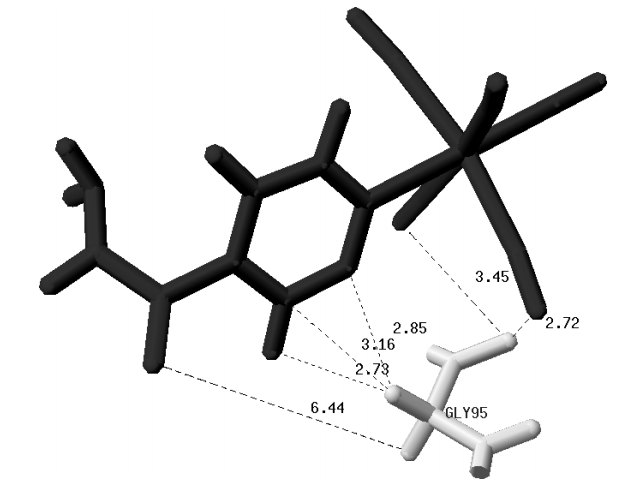
\includegraphics[scale=0.5]{images/distEucli.png}
	\caption{Cálculo das distâncias atômicas entre o ligante PIF (cor preta) e o resíduo GLY95 (cor cinza) do receptor InhA \cite{MAC10}.}
	\label{fig:PIFvsGLY}
\end{figure} 

\section{Identificação dos resíduos relevantes}

Um dos pontos mais importantes para responder aos questionamentos dos especialistas de domínio e fundamental para composição das dimensões, consiste em definir os resíduos mais relevantes para os experimentos de docagem envolvendo os ligantes TCL e ETH com o receptor InhA. 

A enzima InhA é composta de 268 resíduos, e o processo de identificação dos mais importantes leva em consideração o número de contatos estabelecidos entre os átomos do resíduo e o ligante. No \emph{data set} que foi resultado do processo de simulação de docagem, cada átomo do resíduo está representado por uma tripla, contendo a sua localização espacial nos eixos \emph{x, y }e \emph{z}.

De acordo com o especialista de domínio, a interação entre um átomo do resíduo e o ligante só deve ser considerada como contato quando a distância entre ambos seja entre 2{\AA} e 4{\AA}. Valores inferiores a 2{\AA} são descartados por serem considerados uma sobreposição, enquanto valores superiores a 4{\AA} indicam que não foi estabelecido contato. 

Desta forma, para se obter os valores de todo o conjunto presente no \emph{data set} foi calculado a distância Euclidiana tridimensional dos átomos através da equação \ref{eqt:distEuclid}, conforme descrito na seção \ref{sec:IdentificacaoDeMetricas}. Porém, o cálculo foi desconsiderado para todos os átomos de hidrogênio, pois estes devem ser tratados de outra forma.

Portanto, a relevância de um resíduo para um experimento de docagem aumenta em função do número de contatos estabelecidos entre seus átomos e o ligante. As regras de classificação de relevância de um resíduo podem ser sumarizadas da seguinte forma:

\begin{enumerate}
	\item São considerados contatos somente as distâncias entre 2 e 4 {\AA}ngstr\"ons.
	\item Distâncias inferiores a 2 {\AA}ngstr\"ons são desconsideradas.
	\item Átomos de hidrogênio são descartados.
	\item Quanto maior for o número de contatos estabelecidos de um resíduo, mais relevante ele se torna para o experimento.
\end{enumerate}

Além disso, um outro artefato foi utilizado para auxiliar na identificação de resíduos relevantes. Baseado em análises e estudos de experimentos anteriores utilizando a InhA como molécula receptora, um especialista de domínio elaborou uma lista dos 52 principais resíduos que possuem relevância para os experimentos de docagem baseados no mesmo cenário. A Tabela \ref{tab:listaOsmar} lista os resíduos representados pela sua sigla e seu número de ordem na enzima.

\begin{table}[h]
\caption{Lista elaborada pelo especialista de domínio com os principais resíduos para experimentos de docagem utilizando a enzima InhA.}
\label{tab:listaOsmar}
\centering
\begin{tabular}{@{}lllllll@{}}
GLY\_13	&	PHE\_40 &	PHE\_96	&	PHE\_148 &	PRO\_191 &	ILE\_201 &	GLU\_209 		\\
ILE\_14	&	LEU\_62 &	MET\_97	&	PRO\_155 &	ILE\_193 &	VAL\_202 &	ALA\_210 		\\
ILE\_15	&	ASP\_63 &	GLN\_99	&	ALA\_156 &	THR\_195 &	GLY\_203 &	ILE\_214 		\\
THR\_16	&	VAL\_64 &	MET\_102 &	TYR\_157 &	LEU\_196 &	GLY\_204 &	LEU\_217 		\\
SER\_18	&	GLN\_65 &	GLY\_103 &	MET\_160 &	ALA\_197 &	ALA\_205 &					\\
SER\_19	&	SER\_93 &	ILE\_121 &	LYS\_164 &	MET\_198 &	LEU\_206 &					\\
ILE\_20	&	ILE\_94	&	MET\_146 &	ALA\_190 &	SER\_199 &	GLY\_207 &					\\
ALA\_21 &	GLY\_95	&	ASP\_147 &	GLY\_191 &	ALA\_200 &	GLU\_208 &					\\ 
\end{tabular}
\end{table}

%----------------------
%  TO DO: REFERENCIAR ALGORITMO ---------------------------------------
%----------------------
Definido este cenário, foram executados os algoritmos descritos em \ref{alg:CalculoDistancia} para o cálculo das distâncias e sumarização dos dados. Então, após a execução foi possível obter uma listagem de 15 resíduos com maior número de contatos que eram comuns para os experimentos de docagem envolvendo ambos ligantes TCL e ETH. A Tabela \ref{tab:listaProvavelRelevantes} lista os resíduos obtidos pelo algoritmo, que estão representados pela sua sigla e seu número de ordem na enzima.

\begin{table}[h]
\caption{Resíduos identificados pelo algoritmo de classificação por relevância.}
\label{tab:listaProvavelRelevantes}
\centering
\begin{tabular}{@{}lll@{}}
ILE\_15  & ASP\_149 & MET\_160 \\
SER\_19  & ARG\_152 & ILE\_193 \\
ILE\_94  & ALA\_153 & THR\_195 \\
GLY\_95  & MET\_154 & MET\_198 \\
PHE\_148 & TYR\_157 & TRP\_221 \\
\end{tabular}
\end{table}

Com posse destes dados, os resíduos resultantes (apresentados na Tabela \ref{tab:listaRelevantes}) foram comparados com a lista feita pelo especialista de domínio (apresentados na Tabela \ref{tab:listaOsmar}) a fim de identificar os elementos que eram comuns aos dois grupos. 

Os resíduos do conjunto obtido foram plotados pelos especialistas de domínio do LABIO e estão ilustrados pela Figura \ref{fig:PlotResiduos}. Dos 15 resíduos identificados pelo algoritmo, 10 deles estão presentes na lista do especialista de domínio e foram classificados como sendo relevantes para os experimentos de docagem. Os 5 resíduos que não estavam presentes na lista do especialista foram identificados como casos onde a proteína apresentou ligações fora da cavidade do substrato e, por este motivo, não foram considerados como sendo relevantes.

\begin{figure}[h]
        \center
        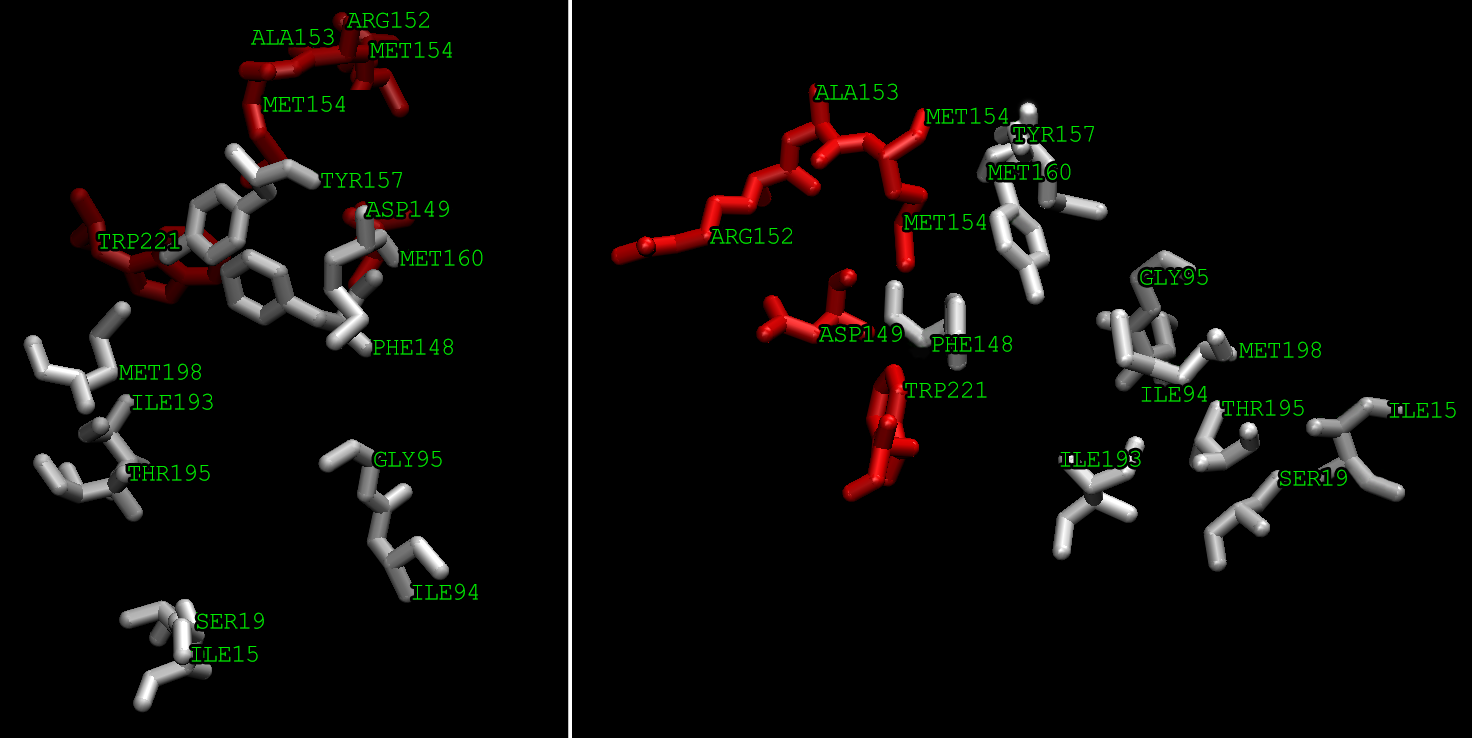
\includegraphics[width=10cm]{images/avaliacao_Residuos_nomes.png}
        \label{fig:PlotResiduos}
        \caption{Plotagem dos 15 resíduos identificados pelo algoritmo de classificação por relevância. A cor cinza representa os resíduos que são relevantes e aparecem na listagem do especialista de domínio, já os resíduos que estão em vermelho não estão presentes na lista.}
\end{figure}

Por fim, com base nestas comparações e nos experimentos realizados foi possível elencar os 10 principais resíduos mais relevantes para responder às questões de negócio. O conjunto final está listado na Tabela

\begin{table}[h]
\caption{Conjunto final de resíduos relevantes para experimentos de docagem molecular considerando como receptor a enzima da InhA e ligantes TCL e ETH.}
\label{tab:listaProvavelRelevantes}
\centering
\begin{tabular}{@{}ll@{}}
\toprule
\multicolumn{1}{c}{Resíduo} & \multicolumn{1}{c}{Nome} \\ \midrule
SER\_19                     & Serina                   \\
ILE\_15                     & Isoleucina               \\
ILE\_94                     & Isoleucina               \\
GLY\_95                     & Glicina                  \\
PHE\_148                    & Fenilalanina             \\
TYR\_157                    & Tirosina                 \\
MET\_160                    & Metionina                \\
ILE\_193                    & Isoleucina               \\
THR\_195                    & Treonina                 \\
MET\_198                    & Metionina                \\ \bottomrule
\end{tabular}
\end{table}

\section{Scripts para preparação dos dados}
\label{sec:ScriptsParaPreparacaoDosDados}

Com objetivo de realizar todo processo de extração, transformação e carga dos dados de simulações de docagem molecular, foram criados quatro \emph{scripts} utilizando as linguagens Python e Bash. Cada script foi criado para atender a uma necessidade específica que surgiu ao longo do projeto. Todos os \emph{scripts} são executados através da CLI e exibem seus resultados diretamente em STDOUT. Estes resultados podem ser redirecionados para outro arquivo através de um \emph{pipe}.

O primeiro \emph{script} criado foi chamado de calculaDistancia, ele foi elaborado com o objetivo de elencar quais são os resíduos mais relevantes, atendendo assim a uma necessidade dos especialistas de domínio. O número de contatos do resíduo com o ligante é a medida qualitativa para elencar quais são estes melhores resíduos. Para identificar se houve contato ou não é necessário realizar o cálculo da distância euclidiana entre resíduo e ligante, conforme descrito na fórmula \ref{eqt:distEuclid}. O calculaDistancia recebe três parâmetros na sua execução, o primeiro é um arquivo texto contendo a lista de resíduos, o segundo é um arquivo texto contendo a lista de ligantes e o terceiro é a base de dados das simulações de docagem molecular no formato CSV. A saída do calculaDistancia é também no formato CSV e é composta do número do snapshot, nome do resíduo, nome do ligante e o resultado do cálculo da distância euclidiana. Um último campo foi adicionado a pedido dos especialistas para classificação da distância euclidiana, se foi menor que 2 ou está entre 2 e 4 {\AA}ngstr\"ons. O algoritmo \ref{alg:CalculoDistancia} demonstra o funcionamento do calculaDistancia.

\renewcommand{\algorithmicfor}{\textbf{para}}
\renewcommand{\algorithmicif}{\textbf{se}}
\renewcommand{\algorithmicthen}{\textbf{então}}
\renewcommand{\algorithmicelse}{\textbf{senão}}
\renewcommand{\algorithmicendif}{\textbf{fim se}}
\renewcommand{\algorithmicendfor}{\textbf{fim para}}
\renewcommand{\algorithmicdo}{\textbf{faça}}

\floatname{algorithm}{Algoritmo}
\begin{algorithm}[H]
\caption{Algoritmo para cálculo da distância}
\label{alg:CalculoDistancia}
{\fontsize{10}{10}\selectfont
\begin{algorithmic}[1]
	\STATE Seja R uma lista de resíduos
	\STATE Seja L uma lista de ligantes
	\STATE Seja D a base de dados dos resultados da simulação de docagem molecular
	\STATE Seja r um resíduo de R
	\STATE Seja l um ligante de L
	\STATE Seja d um \emph{snapshot} da conformação da base D
	\FOR{cada d em D}
		\FOR{cada r em R}
			\FOR{cada l em L faça}
			\IF{r não conter átomo de hidrogênio}
			\STATE Distância $\gets \sqrt{(x - a)^{2} +(y - b)^{2} + (z - c)^{2}}$ 
			\ENDIF
			\IF{Distância menor que 4}
				\IF{Distância menor ou igual a 2}
				\STATE Gravar na saída d, r, l, distancia, classificação menor que 2
				\ELSE
				\STATE Gravar na saída d, r, l, distancia, classificação entre 2 e 4
				\ENDIF
			\ENDIF
			\ENDFOR
		\ENDFOR
	\ENDFOR
\end{algorithmic}
}
\end{algorithm}

O segundo \emph{script} criado foi batizado de ajustaColunasDocking e tem como objetivo realizar a manipulação das colunas contidas no CSV resultante da simulação do processo de docagem molecular. Como o arquivo CSV utilizado possui 12335 colunas, fica difícil realizar a manipulação das mesas através de um software de planilha eletrônica como o \emph{Microsoft Excel}, por exemplo. A necessidade de manipulação destas colunas surgiu após os especialistas de domínio identificarem que o resíduo NAH deveria ter a sua distância euclidiana calculada apenas com o ligante Triclosano. Desta forma foi necessário dividir o arquivo CSV original em dois, um contendo apenas as informações do resíduo NAH e o ligante Triclosano, e o segundo contendo todo o conteúdo original exceto o resíduo NAH. Para esta manipulação o ajustaColunasDocking foi desenvolvido e ele recebe quarto parâmetros de entrada para execução. O primeiro parâmetro é a respeito de qual operação será executada, se serão mantidas apenas as colunas descritas (-m) ou se serão excluída apenas as colunas descritas. O segundo parâmetro é a lista de colunas separadas por vírgula, o terceiro é o arquivo CSV de entrada e o último parâmetro é onde será gravado o novo arquivo. O algoritmo \ref{alg:ajustaColunaDocking} descreve o comportamento do ajustaColunasDocking.

\floatname{algorithm}{Algoritmo}
\begin{algorithm}[H]
\caption{Algoritmo para manipulação da base de dados da simulação de docagem molecular}
\label{alg:ajustaColunaDocking}
{\fontsize{10}{10}\selectfont
\begin{algorithmic}[1]
	\STATE Seja C a lista com o nome das colunas
	\STATE Seja D a base de dados dos resultados da simulação de docagem molecular
	\STATE Seja c uma coluna em C
	\STATE Seja d uma linha em D
	\STATE Seja M o modo de operação da execução
	\IF{M for igual a manter as colunas em C}
		\FOR{cada d em D}
			\FOR{cada c em C}
			\STATE Grave apenas c na saída
			\ENDFOR
		\ENDFOR
	\ENDIF
	\IF{M for igual a excluir as colunas em C}
		\FOR{cada d em D}
			\FOR{cada c em C}
			\STATE Remove apenas c na saída
			\ENDFOR
		\ENDFOR
	\ENDIF
\end{algorithmic}
}
\end{algorithm}

O terceiro script está relacionado com o processo de carga dos dados e foi chamado de criaDadosDIMTempo. O objetivo dele é fornecer o \emph{script} SQL para inserção dos dados na dimensão tempo. O detalhamento a respeito das dimensões será visto na seção \ref{sec:Dimensoes}. O criaDadosDIMTempo recebe apenas um parâmetro de entrada para execução que é o número de picosegundos que vão ser populados na tabela dentro do banco de dados. A saída é um comando de \emph{INSERT} do SQL para gravação na base de dados. O algoritmo \ref{alg:criaDadosDIMTempo} descreve o funcionamento do criaDadosDIMTempo.

\floatname{algorithm}{Algoritmo}
\begin{algorithm}[H]
\caption{Algoritmo para popular os dados na dimensão tempo}
\label{alg:criaDadosDIMTempo}
{\fontsize{10}{10}\selectfont
\begin{algorithmic}[1]
	\STATE Seja P um valor inteiro maior que 1
	\STATE Seja L uma lista de valores
	\STATE Seja c um contador
	\FOR{iteração em P}
		\STATE Incrementa mais um em c
		\IF{c igual a 1000}
			\STATE Armazena o valor de P em L
			\STATE Grave o comando de inserção baseado em L
			\STATE Esvazie L
			\STATE Atribua zero em c
		\ELSE
			\STATE Armazena valor de P em L
		\ENDIF
	\ENDFOR
	\IF{L não estiver vazia}
		\STATE Grave o comando de inserção baseado em L
	\ENDIF
\end{algorithmic}
}
\end{algorithm}

O quarto e último \emph{script} foi chamado de criaDados e é responsável por realizar a carga de todo o restante das informações dentro da base de dados. O criaDados recebe oito parâmetros de entrada para sua execução. Os 4 primeiros parâmetros são referentes a composição das dimensões, que será mais detalhadamente descrito na seção \ref{sec:Dimensoes}. O primeiro parâmetro é um arquivo CSV contendo a composição da dimensão ligante, o segundo referente a dimensão grupo, o terceiro referente a dimensão modelo dinâmico e o quarto referente a composição da dimensão experimento. O quinto parâmetro é o arquivo com a relação dos resíduos mais importantes, o sexto é o arquivo com a relação do número de contatos de cada um dos resíduos. Estas informações foram extraídas após sumarização dos dados de saída do \emph{script} calculaDistancia. O sétimo parâmetro é o arquivo CSV contendo a base de resultados das simulações de docagem molecular. O último parâmetro é um arquivo contendo o agrupamento das conformações existentes no arquivo do parâmetro anterior. A saída do criaDados são os comandos \emph{INSERT} em SQL para popular as informações no banco de dados. O algoritmo \ref{alg:criaDadosFato} descreve o funcionamento do \emph{script} criaDados.

\floatname{algorithm}{Algoritmo}
\begin{algorithm}[H]
\caption{Algoritmo para popular os dados na fato}
\label{alg:criaDadosFato}
{\fontsize{10}{10}\selectfont
\begin{algorithmic}[1]
	\STATE Seja L uma lista de ligantes
	\STATE Seja l um ligante em L
	\STATE Seja G uma lista de grupos
	\STATE Seja g um grupo em G
	\STATE Seja M uma lista de modelos dinâmicos
	\STATE Seja m um modelo dinâmico em M
	\STATE Seja E uma lista de experimentos
	\STATE Seja e um experimento em E
	\STATE Seja R uma lista de resíduos mais importantes
	\STATE Seja r um resíduo em R
	\STATE Seja S uma lista de numero de contato dos resíduos
	\STATE Seja s o numero de um contato em S
	\STATE Seja D a base de dados dos resultados da simulação de docagem molecular
	\STATE Seja d uma conformação em D
	\STATE Seja a um agrupamento de d
	\STATE Seja C uma lista de comandos para inserção
	\FOR{cada l em L}
		\STATE Grave o comando de inserção baseado em l
	\ENDFOR
        \FOR{cada g em G}
		\STATE Grave o comando de inserção baseado em g
        \ENDFOR
        \FOR{cada m em M}
		\STATE Grave o comando de inserção baseado em m
        \ENDFOR
        \FOR{cada e em E}
		\STATE Grave o comando de inserção baseado em e
        \ENDFOR
	\FOR{cada r em R}
		\STATE Grave o comando de inserção baseado em r
	\ENDFOR
	\FOR{cada d em D}
		\STATE Grave a em C
		\FOR{cada l em L}
			\FOR{cada s em S}
				\STATE Gravar o valor de s em C para a composição baseando em d, l e r
			\ENDFOR
			\IF{FEB de d for positiva}
				\STATE Gravar 0 para FEB de d em C
			\ELSE
				\STATE Gravar FEB de d em C
			\ENDIF
			\STATE Gravar RMSD de d em C
			\STATE Gravar o comando de inserção baseado em C
		\ENDFOR
	\ENDFOR
\end{algorithmic}
}
\end{algorithm}

Desta forma o procedimento de execução destas rotinas pode ser definido na seguinte sequência:

\begin{enumerate}
    \item Execução do ajustaColunasDocking para criação de dois arquivos CSV, separando o NAH do restante.
    \item Execução do calculaDistancia para cada um dos arquivos CSV.
    \item Execução do criaDadosDIMTempo para popular a dimensão tempo no banco de dados.
    \item Execução do criaDados para popular o restante das informações no banco de dados.
\end{enumerate}

%-------------------
% TO DO:  mostrar tabela de exemplo do resultado de saída do script.
%-------------------

\section{Dimensões}
\label{sec:Dimensoes}
	mostrar hierarquias de dimensoes
	
\section{Construção do modelo no Analisys Services}
	exibir a tabela pivotante com os valores medios (feb,rmsd)
